\section{Methods}


\subsection{Data set}
Images from the ImageCLEF2012 Plant Identification Task were used in this study~\cite{imageclef2012}.
The data set consists of high resolution colour images that are labelled with metadata such as the full taxon name of the plant, its common name, and the GPS coordinates of the observation.
The images vary in resolution and aspect ratio but are scaled so that their longest axis is 800 pixels.
The data set originally contains three types of images: \emph{scans}, scan-like photographs (\emph{pseudoscans}), and normal \emph{photographs}.
Examples of these three types are shown in Figure~\vref{fig:imagetypes}.
They differ in the complexity of their backgrounds: \emph{scans} have a purely white background and few shadows, whereas \emph{pseudoscans}, while maintaining a uniform background, are more variable in the colour of their background and the lighting conditions.
Finally, \emph{photographs} have very diverse backgrounds, often with other plants visible, and vary strongly in their lighting conditions.


\begin{figure}[htb]
\centering
\resizebox{\textwidth}{!}{
\begin{tabular}{c@{\hskip 0.1in}c|c@{\hskip 0.1in}c|c@{\hskip 0.1in}c}
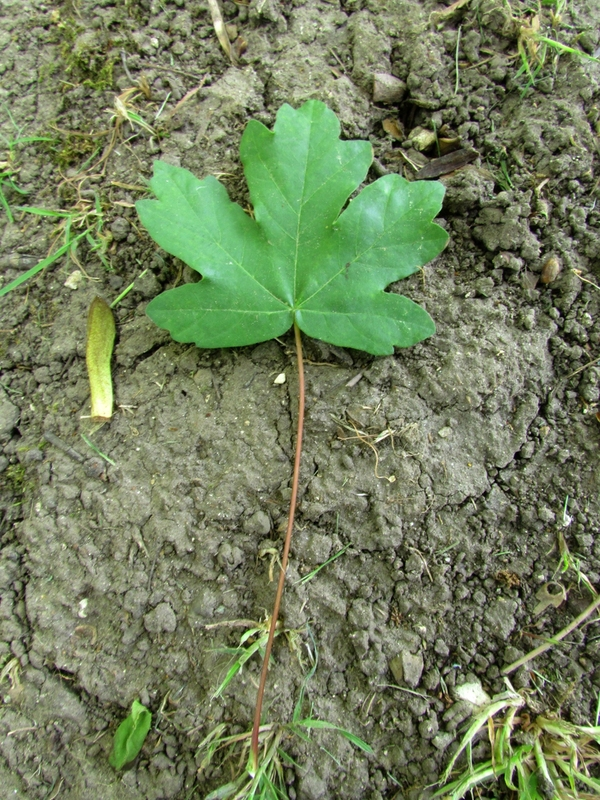
\includegraphics[width = .12\textwidth]{image/10733photograph.jpg} &
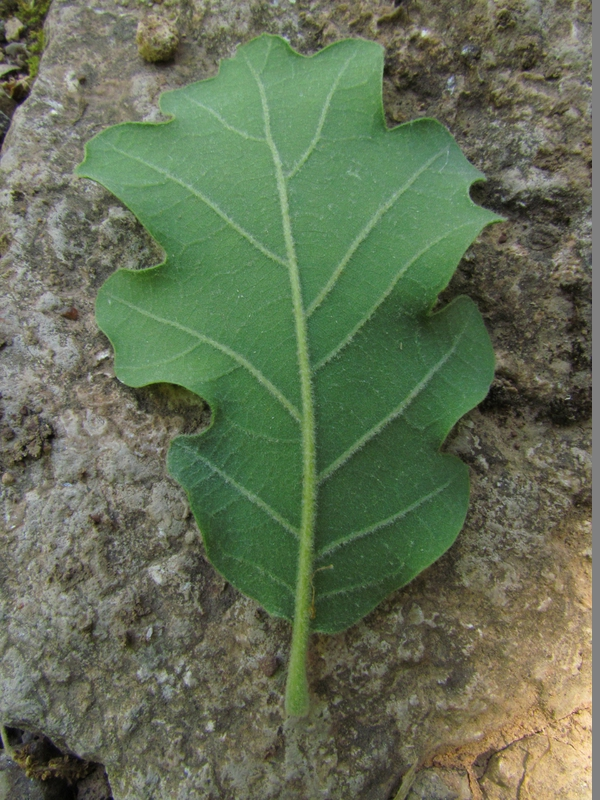
\includegraphics[width = .12\textwidth]{image/3702photograph.jpg} &
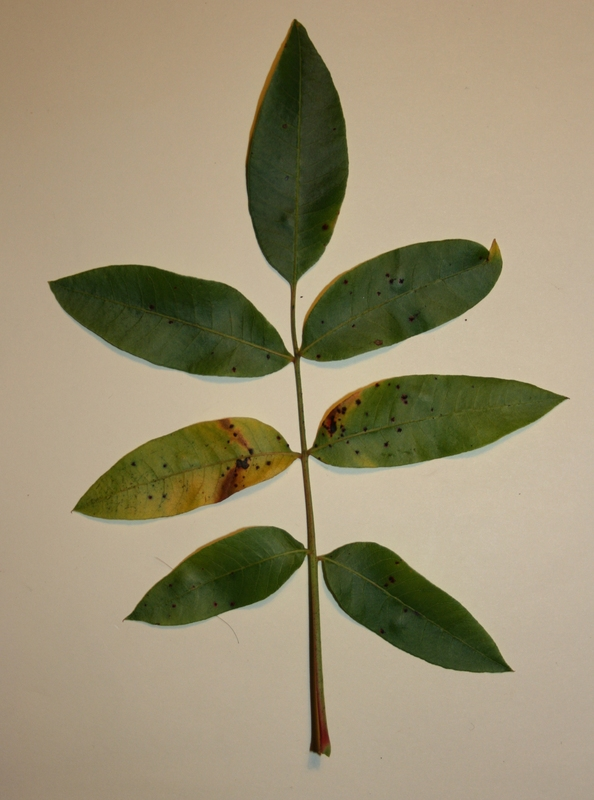
\includegraphics[width = .12\textwidth]{image/10513pseudoscan.jpg} &
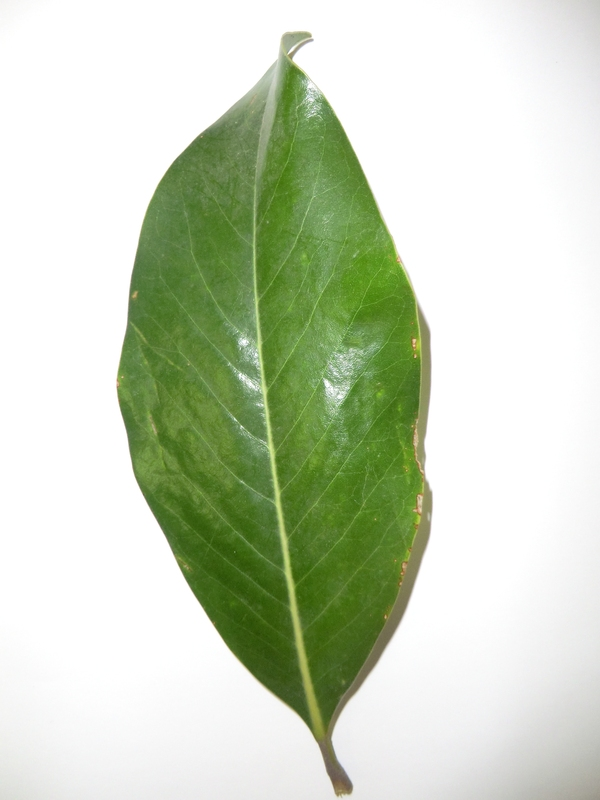
\includegraphics[width = .12\textwidth]{image/10145pseudoscan.jpg} &
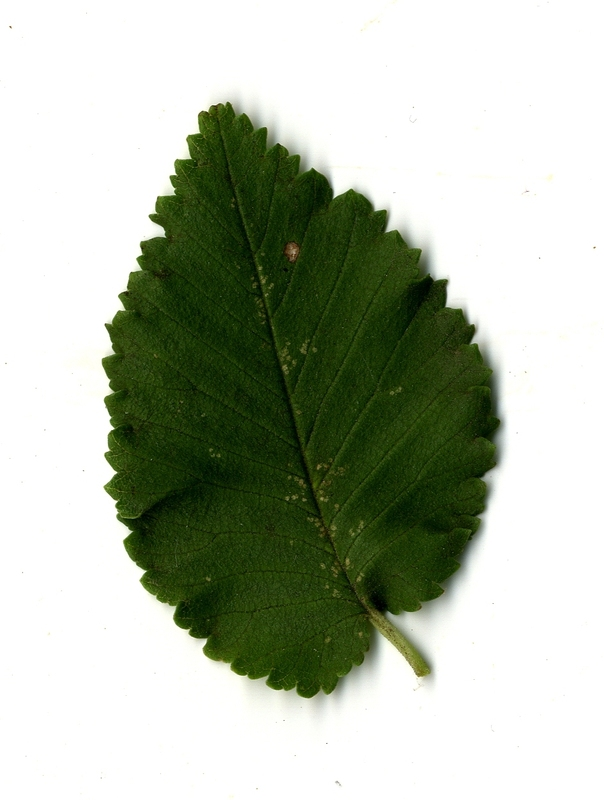
\includegraphics[width = .12\textwidth]{image/4564scan.jpg} &
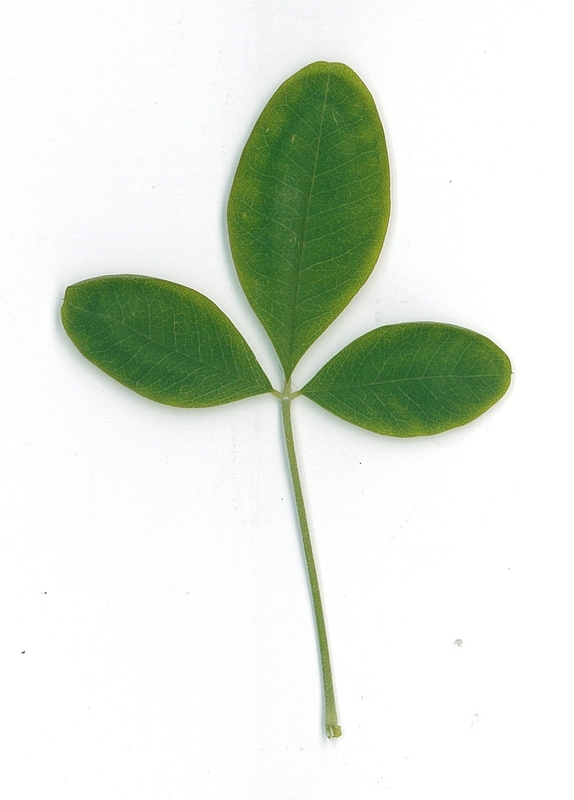
\includegraphics[width = .12\textwidth]{image/725scan.jpg}\\
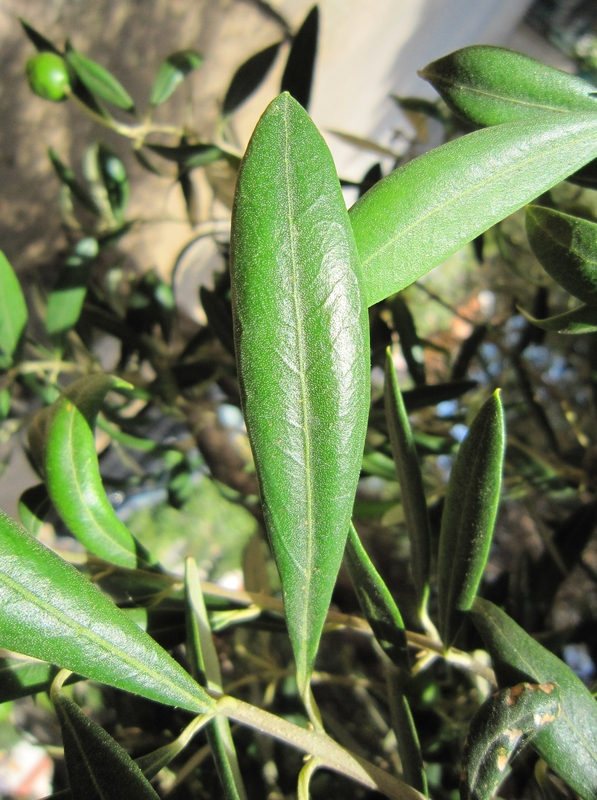
\includegraphics[width = .12\textwidth]{image/3589photograph.jpg} &
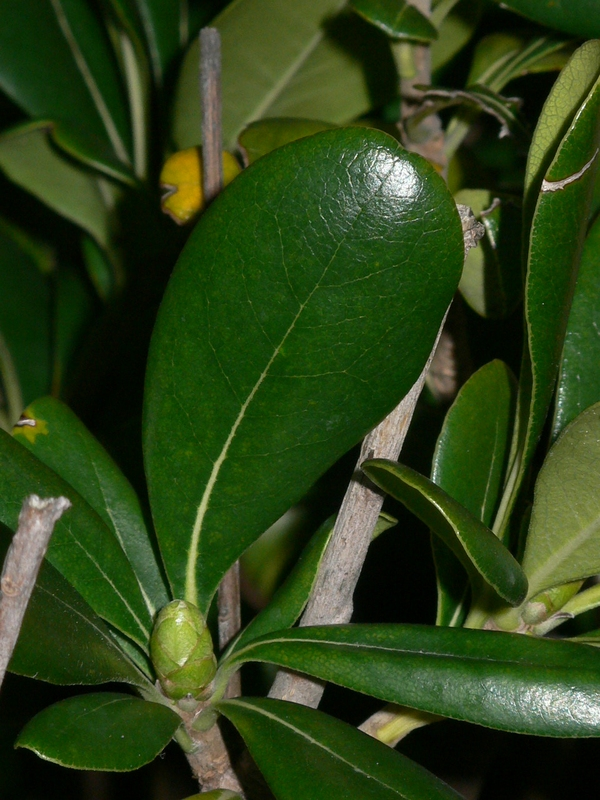
\includegraphics[width = .12\textwidth]{image/4717photograph.jpg} &
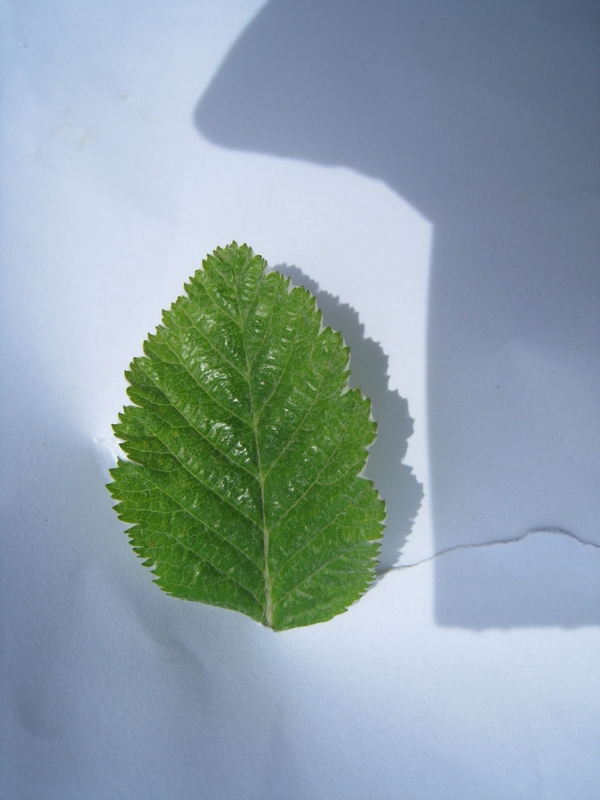
\includegraphics[width = .12\textwidth]{image/5093pseudoscan.jpg} &
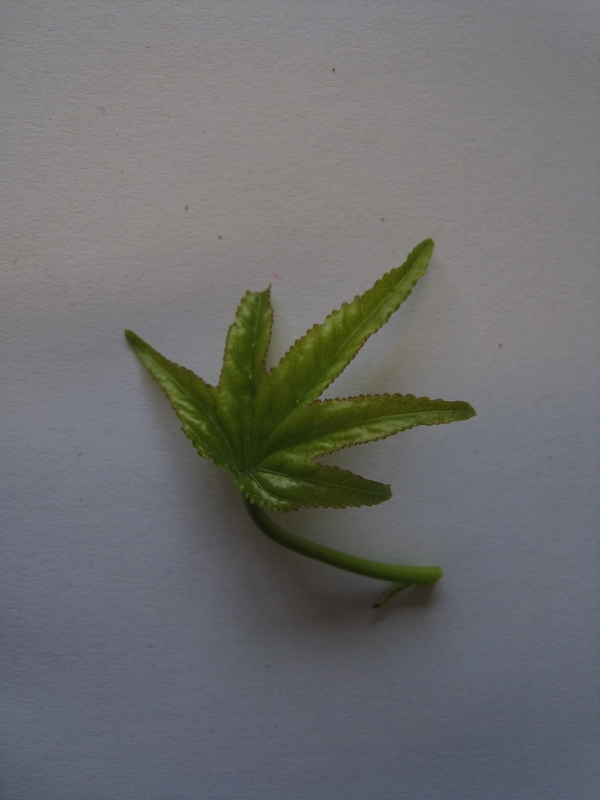
\includegraphics[width = .12\textwidth]{image/2655pseudoscan.jpg} &
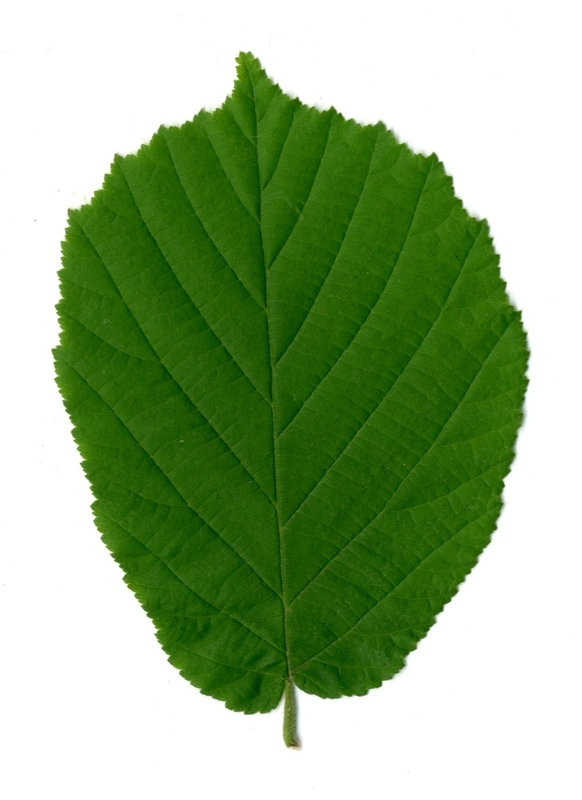
\includegraphics[width = .12\textwidth]{image/8736scan.jpg} &
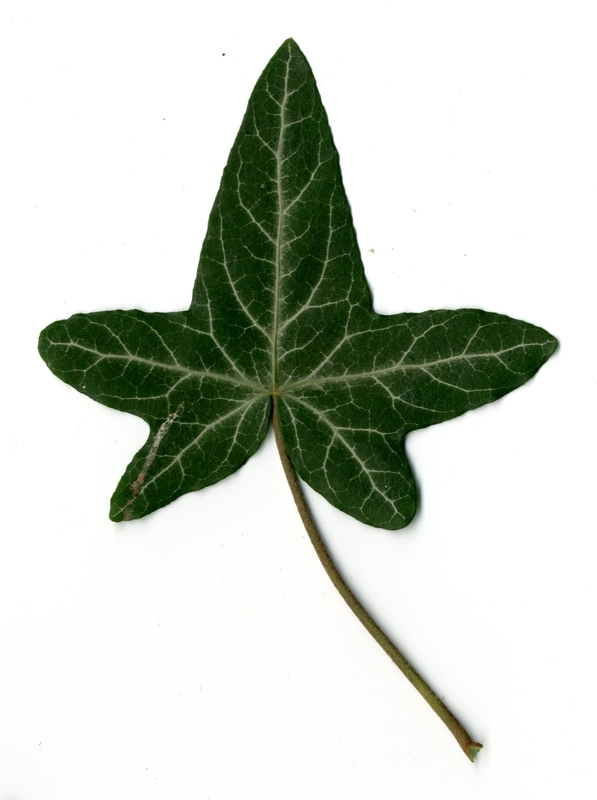
\includegraphics[width = .12\textwidth]{image/5292scan.jpg}
\end{tabular}
}
\caption{Examples of the three image types in the original ImageCLEF2012 data set. From left to right: \emph{photograph}, \emph{pseudoscan}, and \emph{scan}.}
\label{fig:imagetypes}
\end{figure}

Because of the complexity associated with extracting the leaf from its background, only \emph{scan} images (57\% of all images) were used in this study.
This subset consisted of 6630 images of leaves from [??] classes.		%% missing number!
There were [??] images per class on average.	%% missing number!

The images were divided into a training set of 4870 images ($\pm 73\%$) and a test set of 1760 images ($\pm 27\%$).


\subsection{Feature extraction}
Several image classification studies~\cite{Wang2015, Lowe1999}, including at least one study into leaf image classification~\cite{Wang2011}, have made use of Scale-Invariant Feature Transform (SIFT) descriptors.
These descriptors are invariant to changes in scale and rotation, and somewhat robust to variations in viewpoint and illumination.
This makes them suitable for this task, since the leaves are photographed at varying scales and rotations.

% Images are converted to B/W, mask is applied.
% SIFT descriptors are extracted from area not covered by mask (the leaf).
% What does SIFT algorithm do, how does it work?
% Show keypoints in a nice image!
% ...

\subsection{Bag of visual words}


\subsection{Classifiers}
